\documentclass[15pt,a4paper]{article}
\usepackage[pdftex]{graphicx}
\usepackage{graphicx}
\usepackage{amsmath}
\DeclareMathOperator{\Lagr}{\mathcal{L}}
\usepackage{listings}
\usepackage{url}
\usepackage{amsmath}
\usepackage[margin=0.989in]{geometry}
\usepackage[utf8]{inputenc}\Large
\begin{document}
\title{ENDSEM}
\author{JAGAN M J EE20B047}
\maketitle


\section{AIM}
We have to find the antenna currents in a half-wave dipole antenna. For that a long wire carries a current $I(z)$ in a dipole antenna with half length - 0.5m, wavelength - 2m. The standard analysis assumes that the antenna current is given by the equation : \\\\

$
\begin{array}{cc}
I = 
   \Bigg\{ & 
    \begin{array}{cc}
      I_msin(k(l - z)) & 0\leq z\leq l\\
      I_msin(k(l + z)) & -l\leq z\leq 0\\
    \end{array}
\end{array}
$
\\\\\\We have to obtain the expressin for the current vector and see if our answer is matching with the above equation.\\

\section{Calculation of Current and location vector}
The position vectors are $z$ and $u$ whereas current vectors are $I$ and $J$. For calculating the $z$ array and, its given as : 

\begin{equation*}
z[i + N] = \frac{il}{N} , -N\leq i \leq N\\\\\newline
\end{equation*}


For the $u$ array, its divided into two parts : $v$ and $w$ and they are given as \\\\

\begin{equation*}
v[k] = -l + \frac{l}{N} + \frac{kl}{N} ,\>   0\leq k \leq N -2\\\\
\end{equation*}

\begin{equation*}
w[k] =  \frac{l}{N} - \frac{kl}{N} ,\>   0\leq k \leq N -2\\\\
\end{equation*}

This is so to obtain the $u$ array that does not include the end points and the middle point. The array, $u$ is then obtained as shown below: 

\begin{equation*}
u[a] =  v[k]  ,\>   0\leq a \leq N -2,  0\leq k \leq N -2
\end{equation*}

\begin{equation*}
u[a+N-1] =  w[k]  ,\>   0\leq a \leq N -2,  0\leq k \leq N -2
\end{equation*}

The current array $I$ is given $Im = 0.05$ at the middle point ($z = 0$) with rest all the points as 'Zero'. The curent array $J$ is given 'Zero' to all the points.


\section{Calculation of M matrix}

We can compute the M matrix by using Ampere's Law : 













\begin{equation*}
H = M*J 
\end{equation*}





\section{Calculation of $R_z$, $R_u$, $P$ and $P_B$}

For the calculation of vector potential $A(r,z)$, it can further be simplified into a equation consisting of $P$ which is a square matrix of order $2N-2$ and $P_B$ is a column vector. $P_B$ is the contribution to the vector potential due to currrent $I_N$.  $P_B$ is given by : 

\begin{equation*}
P_B = \frac{\mu_0}{4\pi} \frac{exp(-jkR_{iN})}{R_{iN}} dz 
\end{equation*}



Also the vectors $R_z$ and $R_u$ are obtained from the general equation : 

\begin{equation*}
\vec{R} = \vec{r}\hat{r} + (z_i - z_j)\hat{z} 
\end{equation*}

The difference between Rz and Ru is that the former computes
distances including distances to known currents, while Ru is a vector of distances to
unknown currents. Also the matrices $Q$ and $Q_B$ are also calculated.

\section{Final equation and Plot}
The final equation is given by : 

\begin{equation*}
MJ = QJ + Q_B I_M 
\end{equation*}

ie, 

\begin{equation*}
(M-Q)J = Q_B I_M 
\end{equation*}

The value of $J$ can thus be obtained as all other quantities have been obtained in the earlier section. $J$ is the current vector corresponding to unknown currents. From this , $I$ is obtained by adding the boundary conditions  ie zero at i=0, i=2N, and Im at i=N). The following plot gives the variation of $I$ with $z$ and comparison with the assumed equation of $I$\\\\\\\\\\\\\\\\\\\\\\\\\\\\\\\\\\\\\\\\\\\\\\\\\\\\\\

\begin{figure}[!tbh]

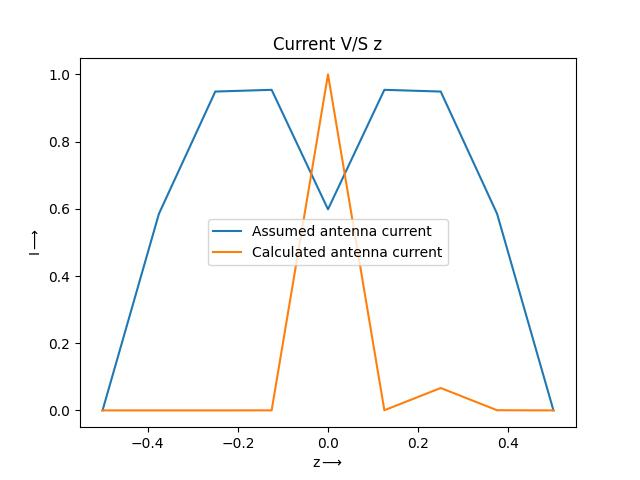
\includegraphics[width = 0.9\textwidth]{latux.jpeg}
\caption{Currents V/S z}

\end{figure}

\section{Conclusion}

We have understood how current flows in a half-wave dipole antenna and compared it with the assumed current flow in it. There's still difference between the two of them but still its an appreciable estimation.







\end{document}